\section{Gebruikers Beschrijving}

\subsection{Belanghebbenden}
In deze sectie van het SRD worden de belanghebbende van de opdracht geïdentificeerd. Er zal ook worden beschreven wat de behoeften zijn van de belanghebbenden, die uiteindelijk zullen worden overwogen in het ontwerpproces.

\textbf{Belanghebbenden:}

\begin{itemize}
	\item \textbf{Customer Service (Hoofdgebruiker van de testkast)}
	\begin{itemize}
		\item De customer serviceafdeling zal de testkast gaan gebruiken om teruggestuurde spindels te testen en te analyseren. De behoeften van deze afdeling zullen zijn:
		\begin{enumerate}
			\item Een gebruiksvriendelijke interface om verschillende spindels te testen op de testkast.
			
			\item De testresultaten moeten betrouwbaar zijn en reproduceerbaar.
			
			\item Log bestanden en testrapporten om analyses uit te voeren.
			
			\item Test criteria waar de motoren aan moeten voldoen zodat ze als goed of slecht kunnen worden bestempeld.
			
			\item Meerdere soorten motoren moeten werken op de testkast.
			
			\item Documentatie om de kast te bedienen.
		\end{enumerate}
	\end{itemize}
	
	\item \textbf{Operators (Dagelijkse gebruikers van de testkast)}
	\begin{itemize}
		\item De operators van de testkast zijn de mensen die de kast daadwerkelijk gaan gebruiken. Hun behoeften kunnen zijn:
		\begin{enumerate}
			\item Een gemakkelijke manier om de testparameters voor een specifieke spindel te selecteren.
			
			\item Een veilig systeem wat de risico’s minimaliseert tijdens het testen van de spindels.
			
			\item Een testproces wat niet te veel tijd kost.
			
			\item Duidelijke feedback van de testkast als eventuele problemen zich voor doen. (Foutmeldingen of waarschuwingen)
			
			\item Eventueel vertaalde tekst op het scherm in andere talen.
		\end{enumerate}
	\end{itemize}
	
	\item \textbf{Onderhoudsdienst}
	\begin{itemize}
		\item De onderhoudsdienst is verantwoordelijk voor het onderhoud van de testkast en eventuele uitbreiding van de kast. De behoeften van deze groep is:
		\begin{enumerate}
			\item Goede documentatie van de code.
			
			\item Inzicht in de parameters en instellingen van de testkast.
			
			\item Goed documentatie van de hardware.
		\end{enumerate}
	\end{itemize}
	
	\item \textbf{R\&D Engineering Team}
	\begin{itemize}
		\item Wanneer Voortman besluit nieuwe machines te ontwikkelen met mogelijk nieuwe type spindels kan de testkast ook nuttig zijn voor de R\&D. Zij zouden de volgende dingen willen:
		\begin{enumerate}
			\item Makkelijk nieuwe testscenario’s kunnen instellen voor de nieuwe motoren.
			
			\item Overzicht over de prestaties van de spindel.
		\end{enumerate}
	\end{itemize}
	
	\item \textbf{Klanten van Voortman}
	\begin{itemize}
		\item Klanten die de gereviseerde motor uiteindelijk kopen kunnen ook baat hebben bij de testkast zij zouden de volgende dingen willen hebben:
		\begin{enumerate}
			\item Een testrapport waarin te zien is dat de gekochte gereviseerde spindel correct werkt naar behoren.
		\end{enumerate}
	\end{itemize}
\end{itemize}

\newpage

\subsection{Gebruikersscenario(s)}

In deze sectie worden alle verschillende gebruikersscenario’s geschetst om de interactie die de gebruiker heeft met het systeem te visualiseren. De volgende stappen moeten doorlopen worden om de spindel juist aan te sluiten en te testen op de testkast.

\begin{figure}[H]
	\centering
	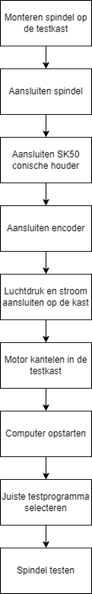
\includegraphics[width=0.18\linewidth]{Gebruikersscenario}
	\label{fig:Gebruikersscenario}
	\caption{Gebruikersscenario spindel bedienen}
\end{figure}

\newpage

\begin{itemize}
	\item \textbf{Monteren spindel op de testkast} houdt in dat de spindel met tenminste twee bouten wordt vastgedraaid op de testkast zodat deze niet meer kan bewegen.
	
	\item \textbf{Aansluiten spindel} betekent dat de drive wordt aangesloten op de spindel.
	
	\item \textbf{Aansluiten SK50 conische houder} betekent dat de luchtcilinders worden aangesloten op de testkast en dat de sensor die checkt of de houder goed gesloten is aangesloten wordt.
	
	\item \textbf{Aansluiten encoder} houdt in dat de encoder wordt aangesloten op de motordrive.
	
	\item \textbf{Luchtdruk en stroom aansluiten op de testkast} houdt in dat de testkast aangesloten wordt op het lichtnet en op de luchtdruk.
	
	\item \textbf{Motor kantelen in de testkast} houdt in dat de spindel wordt gekanteld doormiddel van een Linak actuator binnen in de testkast dit zorgt ervoor dat het draaiende gedeelte van de spindel niet of moeilijker bereikbaar wordt voor de gebruiker dit waarborgt de veiligheid van de gebruiker.
	
	\item \textbf{Computer opstarten} nu alles gereed is kan de computer opgestart worden het testprogramma zou automatisch moeten verschijnen.
	
	\item \textbf{Juist programma kiezen} wanneer de computer is opgestart kan er een testprogramma worden gekozen de juiste parameters worden dan in de drive geladen en de spindel is klaar om getest te worden.
	
	\item \textbf{Spindel testen} de spindel kan nu getest worden.
\end{itemize}

\newpage

\subsection{Voorbeeld eis}

In deze sectie is een kort voorbeeld gemaakt over hoe de eisen in elkaar zitten. Dit is te zien in onderstaande tabel.

\eistabel{Uniek ID}{Titel}{Prioriteit}{Eis van de stelling}{Meetmethode}{Eventuele opmerkingen}

De bovenste rij van de tabel geeft de volgende dingen weer:

\begin{itemize}
	\item \textbf{Uniek ID}
	\begin{itemize}
		\item Elke eis heeft zijn eigen unieke ID zodat hier later naar verwezen kan worden.
	\end{itemize}
	
	\item \textbf{Titel}
	\begin{itemize}
		\item Elke eis heeft zijn eigen titel die kort de eis beschrijft.
	\end{itemize}
	
	\item \textbf{Prioriteit}
	\begin{itemize}
		\item Niet elke eis is urgent en daarom heeft elke eis zijn eigen prioriteit. Er zijn vier prioriteiten: URGENT, HOOG, GEMIDDELD en LAAG.
	\end{itemize}
\end{itemize}

De rest van de tabel omvat het volgende:

\begin{itemize}
	\item \textbf{Stelling}
	\begin{itemize}
		\item Een duidelijke en beknopte beschrijving van de eis.
	\end{itemize}
	
	\item \textbf{Meetmethode}
	\begin{itemize}
		\item Een methode hoe de eis gevalideerd gaat worden in de testfase van het project.
	\end{itemize}
	
	\item \textbf{Opmerking}
	\begin{itemize}
		\item Om onduidelijkheden te verhelpen kan er nog een aanvullende opmerking worden toegevoegd in deze rij.
	\end{itemize}
\end{itemize}

\subsection{Functionele eisen}

\eistabel{FR-001}{Geautomatiseerd testen}{URGENT}{De testkast moet in staat zijn om geautomatiseerd te kunnen testen. Dit houdt in dat er testen gemaakt moeten kunnen worden die vervolgens uitgevoerd kunnen worden op de testkast.}{De eis is behaald wanneer een operator, die los staat van dit project, op de testkast een test kan maken met het instructieboekje en deze ook kan afspelen op de testkast. Deze testkast moet deze test dan automatisch afspelen.}{De operator moet tenminste de keuze hebben uit welk toerental, hoe snel de spindel deze moet bereiken en voor hoelang de spindel moet draaien in dit toerental.}
\eistabel{FR-002}{Testrapport}{GEMIDDELD}{De testkast moet in staat zijn om na afloop van de test een rapport te maken waarin de resultaten van de test staan.}{De eis is behaald wanneer het programma op de testkast een testrapport maakt na afloop van de test. De door de operator gekozen parameters moeten tijdens de test gemonitord worden en weergegeven worden in het rapport. Ook de hoeveelheid samples per seconde moet door de operator gekozen kunnen worden.}{}
\eistabel{FR-003}{Spindel validatie}{LAAG}{Na afloop van de test moet de testkast doormiddel van een statistische analyse van de opgenomen parameters aan kunnen geven of dit binnen de toegestane toleranties en specificaties valt, en of de spindel als ‘goed’ of ‘afgekeurd’ geclassificeerd moet worden.}{De eis is behaald wanneer de testkast spindels kan keuren op basis van tenminste het stroomverbruik deze mag niet significant afwijken van nieuwe spindels met een betrouwbaarheidsinterval van 95\%. De controlegroep moet hiervoor normaal verdeeld zijn met ideaal >30 observaties van nieuwe correct werkende spindels op verschillende toerentallen.}{}
\eistabel{FR-004}{Real time grafieken}{HOOG}{Tijdens de test moeten er op het scherm grafieken komen met real-time data van de spindel. Welke data er op het scherm moet komen moet kunnen worden gekozen door de gebruiker.}{De eis is behaald wanneer de gebruiker een willekeurige parameter kan kiezen en deze kan monitoren op de \gls{gui} tijdens de test. Ook de hoeveelheid samples per seconde moet gekozen kunnen worden door de gebruiker.}{}
\eistabel{FR-005}{Op afstand testen}{GEMIDDELD}{Wanneer de testkast bezig is moet de gebruiker op afstand de testgegevens kunnen bekijken via bijvoorbeeld het \gls{MQTT}-protocol op grafana.}{De eis is behaald wanneer de gebruiker tenminste het stroomverbruik en hoelang het testen nog duurt kan monitoren vanaf een andere laptop die niet is aangesloten op de testkast.}{}
\eistabel{FR-006}{Automatisch parameters inladen}{URGENT}{De testkast moet geautomatiseerd andere parameters in kunnen laden van andere motoren.}{De eis is behaald op het moment dat er een andere motor wordt aangesloten dat de gebruiker slechts door de motor te selecteren in de \gls{gui} de parameters kan inladen in de drive die passen bij die motor.}{}
\eistabel{FR-007}{Handmatig testen}{URGENT}{De gebruiker moet de spindels handmatig kunnen aansturen met de \gls{gui} op de testkast. }{Deze eis is behaald wanneer de gebruiker handmatig de motor kan aansturen met de \gls{gui} op de testkast.}{Het aansturen kan bijvoorbeeld met een slider.}
\eistabel{FR-008}{TwinSAFE geconfigureerd}{GEMIDDELD}{De veiligheidskritieke onderdelen in de testkast zoals de deurschakelaars maar ook de motordrive moeten worden geconfigureerd in een TwinSAFE project zodat de veiligheid van de gebruiker te allen tijde kan worden gewaarborgd.}{Deze eis is behaald wanneer de motor automatisch en gecontroleerd wordt afgeremd met een TwinSAFE project zodra één van de volgende veiligheidsvoorwaarden worden geactiveerd:
\begin{itemize}
	\item Deurbeveiliging: op het moment dat er een deur op de testkast geopend wordt.
	\item Noodstop: wanneer de noodstop wordt ingedrukt.
	\item Wanneer veiligheidslimieten worden overschreden: Bijvoorbeeld een te hoge stroomafwijking.
\end{itemize} De motor moet zo snel mogelijk afremmen. Omdat dit sterk afhankelijk is van welk type motor en welke massatraagheid de spindel heeft en mogelijk nog de tool die hierin zit kan hier geen vaste waarde aan gehangen worden.}{Momenteel is deze veiligheid al wel ingebouwd in de testkast echter is dit niet gedaan met TwinSAFE maar gewoon geprogrammeerd in een \gls{TwinCAT} \gls{PLC} project. }
\eistabel{FR-009}{Servo Motoren}{URGENT}{Tenminste de volgende motoren moeten kunnen worden aangestuurd door de AX5140 motordrive:
\begin{itemize}
	\item MAD100D-0250-SA-C0-AK0-35-N3 (V623) Async servo motor
	\item MAD130C-0150-SA-S2-AP0-05-N1 (V633, V310 nieuw) Async servo motor
	\item HQL100X (V310 oud) Async servo motor
	\item MSK101D-0450-NN-M1-AP0-NNNN (V505-250T, V320, V330C, V320C en V600) Sync servo motor
	\item MS2N10-D0BNN-AMVK0-NNNNN-NN (V630 nieuw)  Sync servo motor
	\end{itemize}}{Deze eis is behaald wanneer bovenstaande motoren aangestuurd kunnen worden vanaf de drive de motoren moeten hierbij draaien.}{Het aansturen kan bijvoorbeeld met een slider.}
\eistabel{FR-010}{FFT-analyse}{LAAG}{De Testkast moet een Fast Fourier Analysis (\gls{FFT}) kunnen uitvoeren op de gemeten trilling gegevens om frequentiespectra te genereren.}{De eis is behaald wanneer de testkast de spindel die getest wordt kan vergelijken met een aantal juist werkende spindels op basis van de trillingen van de motor en ook kan aangeven waar de verschillen zitten om zo mogelijke problemen aan te kunnen duiden.
	
	\vspace{0.5cm}
Meet eerst de trillingen van de motor bij 20\%, 50\% en 80\% van de maximum snelheid.

Voer de fourier transformatie uit op de samples. De formules hiervan zijn te vinden in bijlage \ref{sec:FourierTransform}.

De Referentie $X_k$ is betrouwbaarder wanneer hier een gemiddelde van wordt genomen met ideaal meer dan 30 samples maar aangezien dit veel tijd kan kosten is het ook al waardevol om dit met minder spindels te doen. Dit gemiddelde kan berekend worden met de volgende formule:

\begin{equation}
	\bar{X}_k=\frac{1}{M}\sum_{i=1}^{M}X_{i,k}
\end{equation}

$M$ is hier het aantal referentie metingen (aantal juiste spindels)

Vervolgens om aan te geven hoeveel afwijking er mag zijn bij goede spindels kan de standaarddeviatie per frequentie worden berekend met de volgende vergelijking:

\begin{equation}
	\sigma_k=\sqrt{\frac{1}{M}\sum_{i=1}^{M}(X_{i,k}-\bar{X}_k)^2}
\end{equation}

De testkast moet vervolgens de verschilspectra laten zien door een soort heat map te laten zien waar de grootste afwijkingen zitten dit kan makkelijk met de volgende formule:

\begin{equation}
	\Delta X_k=\frac{|X_{gereviseerd,k} - \bar{X}_k|}{\sigma_k}
\end{equation}

Dit geeft de afwijking in termen van de standaarddeviatie per frequentie. Als $\Delta X_k$ nu groter is dan 2 betekend dit dat het meer dan 2x de standaarddeviatie is. Dit kan betekenen dat de trillingen te veel afwijken bij een bepaalde frequentie van een normale spindel bij een bepaalde frequentie wat kan wijzen op problemen \cite{web:FLUKE}. 

}{Mochten de frequenties nou erg afwijken in de tijd kan er ook mogelijk een spectrogram gemaakt worden in de tijd of eventueel tegen de motorsnelheid in plaats van de tijd.
\gls{STFT} (Short Time Fourier Transform) \cite{web:STFT} .
Door de PLC cycle snelheid zou de sampling frequentie niet zo hoog kunnen zijn dit zal voor de test betekenen dat hogere frequenties niet kunnen worden geanalyseerd omdat hier aliasing zal optreden.
}
\eistabel{FR-011}{\gls{MCSA} (Motor Current Signature Analysis)}{MEDIUM}{De testkast moet een \gls{FFT} kunnen uitvoeren op de meet gegevens van alle fasen van de motor als functie van de tijd om wikkelfouten, lager schade of speling te analyseren.}{De eis is behaald als de testkast de spindel die getest wordt kan vergelijken met een aantal juist werkende spindels op basis van de variatie in stroom per fase van de motor. De methode hiervan is grotendeels hetzelfde als FR-010 en zal daarom niet uitgebreid uitgelegd worden hieronder.

\vspace{0.5cm}

Meet de stroom per fase bij de in FR-010 beschreven snelheden en pas de \gls{DFT} hierop toe om de volgende data reeksen te krijgen: $I_U\left(\mathcal{F}\right)$, $I_V\left(\mathcal{F}\right)$ en  $I_W\left(\mathcal{F}\right)$ bij elke snelheid.

\vspace{0.5cm}

Gebruik net als bij de trillingen meerdere juist werkende motoren om een gemiddeld spectrum te krijgen met daarbij de standaarddeviatie per frequentie.

\vspace{0.5cm}

${\bar{I}}_U\left(\mathcal{F}\right), {\bar{I}}_V\left(\mathcal{F}\right)$ en ${\bar{I}}_W\left(\mathcal{F}\right)$

\vspace{0.5cm}

${\sigma I}_U\left(\mathcal{F}\right), {\sigma I}_V\left(\mathcal{F}\right)$ en $\sigma I_W\left(\mathcal{F}\right)$

\vspace{0.5cm}

Er moeten vervolgens drie heatmaps gemaakt worden voor elke fase één van de gestandaardiseerde afwijking per frequentie met de volgende formules:

\begin{equation}
	\Delta I_U\left(\mathcal{F}\right)=\frac{\left|{I_U\left(\mathcal{F}\right)}_{gereviseerd}-{\bar{I}}_U\left(\mathcal{F}\right)\right|}{{\sigma I}_U\left(\mathcal{F}\right)}
\end{equation}

\begin{equation}
	\Delta I_V\left(\mathcal{F}\right)=\frac{\left|{I_V\left(\mathcal{F}\right)}_{gereviseerd}-{\bar{I}}_V\left(\mathcal{F}\right)\right|}{{\sigma I}_V\left(\mathcal{F}\right)}
\end{equation}

\begin{equation}
	\Delta I_W\left(\mathcal{F}\right)=\frac{\left|{I_W\left(\mathcal{F}\right)}_{gereviseerd}-{\bar{I}}_W\left(\mathcal{F}\right)\right|}{{\sigma I}_W\left(\mathcal{F}\right)}
\end{equation}

Wanneer een waarde hoger is dan 2 op een bepaald punt kan dit wijzen op een significante afwijking ten opzichte van de juiste spindels. Afwijkingen in de frequentie van de stroom kunnen duiden op asymmetrie, magneetschade (bij synchrone motoren), slechte wikkelingen of een ongelijke belasting. 

}{Mochten de frequenties nou erg afwijken in de tijd kan er ook mogelijk een spectrogram gemaakt worden in de tijd of eventueel tegen de motorsnelheid in plaats van de tijd. (\gls{STFT}) \cite{web:STFT}
Door de \gls{SoE} communicatiesnelheid en de \gls{PLC} cyclus snelheid zou de sampling frequentie niet zo hoog kunnen zijn dit zal voor de test betekenen dat hogere frequenties niet kunnen worden geanalyseerd omdat hier aliasing zal optreden.
}
\eistabel{FR-012}{\gls{RMS} (Root Mean Squared) of the motor vibration}{MEDIUM}{De testkast moet aan kunnen geven of de spindel gemiddeld gezien significant meer trilt dan de referentie spindel.}{De eis is behaald wanneer de testkast de gemeten trillingen vergelijkt met de referentie spindel metingen. Dit kan worden berekend op de volgende manier:
	
	Om te weten of de spindel meer of minder trilt kan worden gebaseerd op de RMS-waarde van de sample de formule hiervoor is als volgt:
	
	\begin{equation}
		X_{RMS}=\sqrt{\frac{1}{n}\sum_{i=0}^{n-1}X_i^2}
	\end{equation}
	
	
	Deze waarde van de gereviseerde spindel mag niet te veel afwijken van de gemiddelde waarde van de referentiegroep (juist werkende spindels) +- 2x de standaarddeviatie hiervan. Waarbij de sample grootte van de referentiegroep ideaal >30 is om zo een normaalverdeling te hebben echter kan dit erg veel werk zijn een lagere sample grootte is daarom ook al waardevol.
	
	De volgende vergelijking kan gebruikt worden om de standaarddeviatie te berekenen van de controlegroep:
	
	\begin{equation}
		\sigma_{RMS}=\sqrt{\frac{1}{N}\sum_{i=0}^{N}\left(X_{i,RMS}-{\bar{X}}_{RMS}\right)^2}
	\end{equation}
	
	
	Hier kunnen we een getal mee berekenen die de gebruiker verteld hoeveel de $X_{RMS}$ van de geteste spindel van het gemiddelde zit van de controlegroep met de volgende formule:
	\begin{equation}
		\Delta X_{RMS}=\frac{X_{RMS,gereviseerd}-{\bar{X}}_{RMS}}{\sigma_{RMS}}
	\end{equation}
	 Wanneer de $\left|\Delta X_{RMS}\ \right|$ groter is dan 2 betekend dit dat het verschil significant is en dat er mogelijk een probleem is. Met uitzondering van wanneer $\Delta X_{RMS}$ negatief is dit zou namelijk betekenen dat de trilling minder is geworden ten opzichte van de control groep na het reviseren.
}{}
\eistabel{FR-013}{Thermische analyse}{LAAG}{De testkast moet op basis van de temperatuur van de motor kunnen beoordelen of deze afwijkt van de toegestane waarden. De testkast moet op dat moment een waarschuwing geven en moet hiernaast ook de temperatuur statistisch vergelijken met de temperatuurdata van goed functionerende spindels, zodat de testkast kan aangeven of de afwijking significant is. Dit maakt het mogelijk om te detecteren of de motor mogelijk te zwaar loopt of andere mankementen.}{
Deze eis is behaald op het moment dat de testkast kan aangeven dat: 

\begin{itemize}
	\item De gemeten temperatuur van de motor significant afwijkt van de controle groep.
	
	\item Op basis van statistische vergelijking wordt een inschatting gemaakt of de motor mogelijk te zwaar loopt.
\end{itemize}

\textbf{Meet methode:}

De motor draait op de volgende snelheden voor 10 minuten:

\begin{itemize}
	\item 20\% maximum snelheid
	\item 50\% maximum snelheid
	\item 80\% maximum snelheid
\end{itemize}

De temperatuur wordt minstens elke seconde opgenomen bij zowel de control groep als de gereviseerde spindel. Vervolgens wordt per seconde het gemiddelde berekent van alle spindels in de controle groep en ook de standaard deviatie met de volgende formules:

\begin{equation}
	\bar{T}_{controle}=\frac{1}{N}\sum_{n=0}^{N-1}T_n
\end{equation}

\begin{equation}
	\sigma_{controle}=\sqrt{\frac{1}{N-1}\sum_{n=0}^{N-1}(T_n-\bar{T}_{controle})^2}
\end{equation}

Vervolgens kan er een tabel gemaakt worden van het genormaliseerde temperatuurverschil met de volgende formules:

\begin{equation}
	\Delta T= T_{gereviseerd} - \bar{T}_{controle}
\end{equation}

\begin{equation}
	Z=\frac{\Delta T}{\sigma_{controle}}
\end{equation}

Wanneer er ergens een waarde hoger is dan 2 dan betekent dit dat de waarde significant afwijkt van de controle groep het kan dan zijn dat er iets aan de hand is.

}{Het aansturen kan bijvoorbeeld met een slider.}
\eistabel{FR-014}{Reset}{URGENT}{Wanneer de reset knop is ingedrukt moeten alle foutmeldingen in het systeem gereset worden waardoor het programma kan vervolgen.}{Wanneer de reset knop is ingedrukt moet de testkast gereset worden dit houdt in dat alle foutmeldingen en ook de drive gereset worden. De drive kan gereset worden door \texttt{0b00000010} big endian naar S-0-0099 in de drive te schrijven.}{}
\eistabel{FR-015}{Stoppen}{URGENT}{Wanneer de stopknop ingedrukt wordt moet het testprogramma dat aan het runnen is onderbroken worden en de spindel moet dan tot stilstand komen.}{De eis is behaald op het moment dat het testprogramma onderboken wordt wanneer de stopknop ingedrukt wordt. De spindel moet op dit moment tot stilstand komen.}{}
\eistabel{FR-016}{Emergency stop}{URGENT}{Wanneer de emergency stop ingedrukt wordt of wanneer de deur van de testkast geopened wordt moet de spindel in \gls{STO} gaan en de safety card in de drive moet op dit moment active worden. Ook mag de toolchanger op dit moment niet meer werken zolang de emergency stop ingedrukt is.}{Deze eis is behaald op het moment dat alle bewegende delen in de testkast stoppen op het moment dat de noodstop is ingedrukt.}{}
\eistabel{FR-017}{Starten}{URGENT}{Waneer de startknop in gedrukt is moet het testprogramma beginnen met lopen.}{Deze eis is behaald op het moment dat het testprogramma begint met afspelen wanneer de startknop is ingedrukt.}{}




